
\chapter{ABORDAGEM PROPOSTA}

Este capítulo detalha a execução prática da metodologia proposta, abrangendo desde o fluxo operacional e as ferramentas utilizadas até o treinamento dos modelos preditivos de classificação e o gerenciamento do projeto.


\section{ANÁLISE EXPLORATÓRIA DE DADOS (EDA)}

A aplicabilidade da técnica de Análise Exploratória de dados apresentou informações relevantes para este estudo. Em um primeiro momento foi extraída a matriz de correlação linear entre variáveis dos indicadores IDSC e o índice do IDEB. A análise da matriz de correlação evidenciou que os indicadores socioeconômicos apresentam associação com o índice do IDEB, porém essa análise identifica apenas relações lineares, se faz necessário o uso de modelos para identificar relações não lineares. A Figura~\ref{fig:heatmapideb} apresenta a matriz de correlação das variáveis citadas.

\begin{figure}[tbph]
	\centering
	\caption{Matriz de correlação linear entre indicadores do IDSC e o IDEB.}
	\label{fig:heatmapideb}
	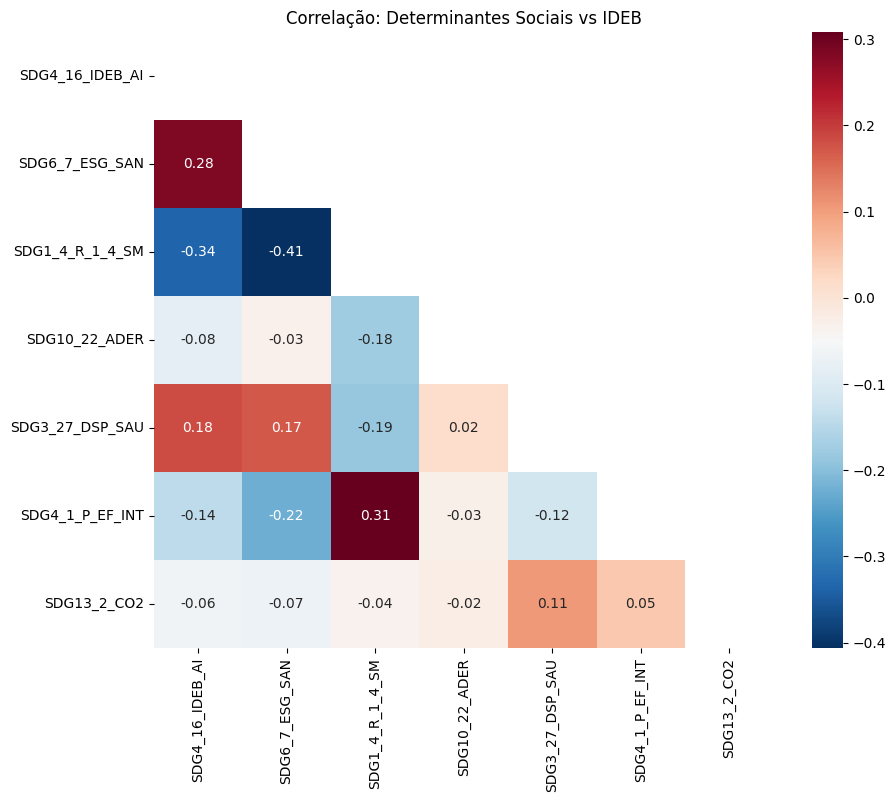
\includegraphics[width=0.7\textwidth]{heat_map_ideb}
	\\ \vspace{2pt} 
	\footnotesize{Fonte: A autora, 2026.}
\end{figure}

Conforme observado na Figura~\ref{fig:scatterideb}, ao lado esquerdo do gráfico o cenário de menor vulnerabilidade socioeconômica apresenta maior dispersão de dados, isso indica que ao estabilizar a renda da população outros fatores possuem maior importância no desempenho do índice de qualidade da educação básica. A linha de tendência central tenta resumir o comportamento nacional, levando em conta todos os municípios presentes na base completa, mas não abrange dados de municípios que se comportam como \textit{outliers} positivos.


\begin{figure}[tbph]
	\centering
	\caption{Gráfico de dispersão entre o indicador de Baixa Renda (eixo x) e o IDEB (eixo) com linha de tendência linear.}
	\label{fig:scatterideb}
	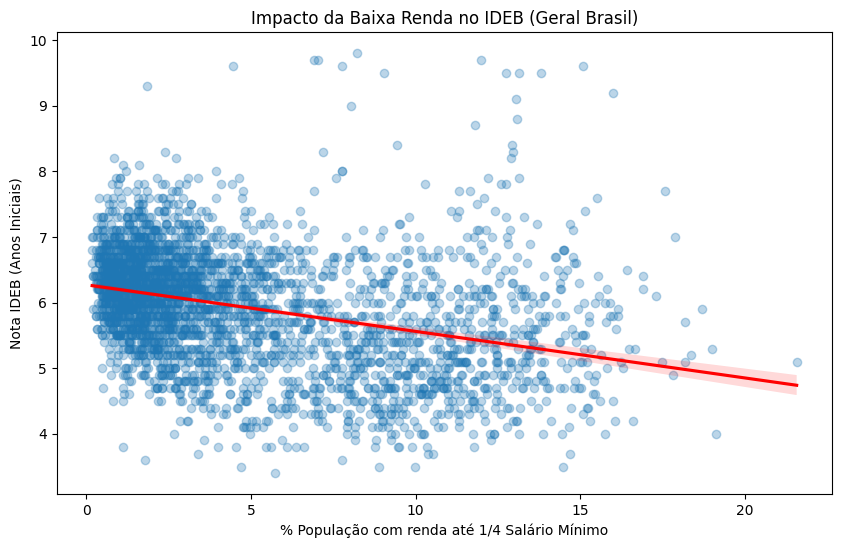
\includegraphics[width=0.8\textwidth]{scatter_ideb}
	\\ \vspace{2pt} 
	\footnotesize{Fonte: A autora, 2026.}
\end{figure}

A Análise Exploratória de Dados evidencia o comportamento da base de dados, demonstrando heterogeneidade dos dados dos municípios brasileiros. Esse comportamento demanda uma estratégia de segmentação da base, no caso deste estudo, a seleção do suconjunto de municípios do estado de Santa Catarina. 

 \section{PRÉ-PROCESSAMENTO DA BASE DE DADOS}
	
Nesta etapa, foram aplicadas técnicas sistemáticas de pré-processamento de dados com o objetivo de estruturar e adequar a base de dados do IDSC-BR para a execução dos algoritmos de aprendizado de máquina. Inicialmente, realizou-se a inspeção do conjunto de dados para a identificação de metadados, colunas descritivas e variáveis categóricas irrelevantes para o processo de predição. Uma etapa metodológica adotada nesta fase foi a remoção preventiva de colunas e índices que pudessem induzir ao vazamento de dados (\textit{data leakage}). Para isso, foram removidas variáveis e notas intermediárias que compartilhavam dependência semântica com as notas e faixas do IDEB, assegurando que os modelos de classificação fossem treinados estritamente com base nos indicadores exógenos de desenvolvimento sustentável, sem variáveis que gerassem acurácias artificialmente infladas. Por fim, após a conclusão da limpeza de dados, a base de dados resultante foi convertida e persistida no formato CSV (\textit{Comma-Separated Values}), otimizando o fluxo de leitura computacional para as etapas subsequentes de modelagem.


\section{TREINAMENTO DOS MODELOS}

Após a realização da etapa de pré-processamento da base de dado, a predição do índice do IDEB foi formulada como um problema de classificação multiclasse. Nessa tarefa, os indicadores do IDSC atuam como atributos preditores e a a faixa de desempenho do município na nota do IDEB, como variável alvo. Sendo assim, foram considerados duas variáveis alvo independentes: Anos Iniciais (AI) e os Anos Finais (AF) do ensino fundamental. Os modelos foram treinados e avaliados separadamente para cada variável. 


\subsection{Definição das classes}

Levando em conta que o IDEB é uma variável contínua, a nota bruta normalizada em uma escala de 0 a 10 foi distribuída em cinco faixas de desempenho:

\begin{itemize}
	\item \textbf{Classe 1 (Insuficiente):} notas inferiores a 4,0;
	\item \textbf{Classe 2 (Básico):} notas entre 4,0 e 4,9;
	\item \textbf{Classe 3 (Intermediário):} notas entre 5,0 e 5,9;
	\item \textbf{Classe 4 (Adequado):} notas entre 6,0 e 6,9;
	\item \textbf{Classe 5 (Avançado):} notas maiores ou iguais a 7,0.
\end{itemize}

Para treinamento do modelo a nota bruta e as classificações do Painel do IDSC-BR não foram utilizadas como atributos, mantidas em arquivo separado. É válida a explicação de que a variável de classificação Painel, que classifica o desempenho dos indicadores em cores não foi utilizada pois alguns municípios não possuiam valor da variável alvo, por isso foi feita a classificação com a nota bruta, abrangendo todos os muniípios. Essa escolha preserva a escala original do índice e dispensa a categorização em quatro cores definida pelo IDSC-BR. A classificação do Painel não foi avaliada como alvo alternativo. Ressalta-se que ela abrange os mesmos municípios que a nota bruta, de modo que a escolha não decorre de diferença de cobertura.

Dos 295 municípios catarinenses, foram mantidos apenas aqueles com IDEB divulgado para a etapa correspondente: 152 nos anos finais e 273 nos anos iniciais. Em seguida, como o estudo se restringe a Santa Catarina, algumas faixas não possuem representantes suficientes. Os municípios pertencentes a classes com menos de dois exemplos foram removidos, pois inviabilizavam a divisão estratificada entre treino e teste. Nos anos finais, foi removido um município da faixa avançada, restando quatro classes e 151 municípios. Nos anos iniciais, foi removido um município da faixa básica e nenhum município se enquadrou na faixa insuficiente, restando três classes e 272 municípios. A Tabela~\ref{tab:distribuicao-classes} apresenta a distribuição final das classes em cada alvo.

\begin{table}[htbp]
	\centering
	\caption{Distribuição dos municípios catarinenses por faixa do IDEB, após os filtros aplicados.}
	\label{tab:distribuicao-classes}
	\begin{tabular}{llrr}
		\toprule
		\textbf{Etapa} & \textbf{Faixa do IDEB} & \textbf{Municípios} & \textbf{\%} \\
		\midrule
		\multirow{4}{*}{Anos finais (n = 151)}
		& Insuficiente (< 4,0)  & 7  & 4,6 \\
		& Básico (4,0--4,9)     & 55 & 36,4 \\
		& Intermediário (5,0--5,9) & 75 & 49,7 \\
		& Adequado (6,0--6,9)   & 14 & 9,3 \\
		\midrule
		\multirow{3}{*}{Anos iniciais (n = 272)}
		& Intermediário (5,0--5,9) & 65  & 23,9 \\
		& Adequado (6,0--6,9)      & 176 & 64,7 \\
		& Avançado ($\geq$ 7,0)    & 31  & 11,4 \\
		\bottomrule
	\end{tabular}
\end{table}

\subsection{Partição dos dados}

Como foi explicado anteriormente, dos 295 municípios catarinenses presentes no IDSC-BR 2025, foram utilizados apenas aqueles com IDEB divulgado para a etapa correspondente e pertencentes a classes com ao menos dois exemplos, resultando em 151 municípios para os anos finais (AF) e 272 para os anos iniciais (AI), conforme a Tabela~\ref{tab:distribuicao-classes}.

A base de dados abrange 151 municípios para os anos finais (AF) e 272 para os anos iniciais. Sendo assim, para cada alvo, os dados foram divididos em 80\% para treino e 20\% para teste, divididos pela classe e com semente aleatória fixa (\textit{random\_state} = 42), garantindo a reprodutibilidade dos resultados. Nesse cenário, a variável alvo dos AF ficou com 120 municípios para treino e 31 para teste, e a variável alvos dos AI, com 217 para treino e 55 para teste. O conjunto de teste foi mantido isolado durante o ajuste de hiperparâmetros e usado apenas na avaliação final. 

Em razão do tamanho reduzido da base, a classificação incorreta de um único município altera a acurácia em aproximadamente 3,2 pontos percentuais no alvo AF e 1,8 ponto percentual no alvo AI. Além disso, as classes menos frequentes ficam com menos exemplos no teste, no contexto desse estudo na variável AF, a classe insuficiente, com 7 municípios, tem apenas um ou dois no conjunto de teste, o que torna as métricas mais instáveis. Esses aspectos limitam a precisão das comparações entre modelos e são considerados na análise dos resultados.

\subsection{Seleção de atributos}

Como comparação de resultados dos modelos treinados com a base de dados com todos os atributos preditores, exceto os alvos e o identificador do município foi realizado um experimento adicional, o treinamento do modelo com um subconjunto de 105 atributos resultante da seleção descrita a seguir. A primeira etapa de filtragem ocorreu por meio de uma análise exploratória, com base na matriz de correlação de Pearson, foram identificados 15 pares de variáveis com correlação absoluta superior ao valor de 0,80, devido a alta correlação, em cada par, foi descartada a variável com maior correlação média que as demais, a primeira etapa já rediziu o conjunto de variáveis preditoras de 135 para 121 colunas. Na etapa subsequente, foram removidas as variáveis relacionadas à educação e ao próprio IDEB (indicadores do ODS 4), evitando que a resposta fosse inferida de atributos semanticamente dependentes do alvo, o que resultou em 105 atributos. Além das duas etapas foi aplicada a Análise de Componentes Principais (PCA) sobre os dados padronizados, com imputação pela mediana dos valores, com 15 componentes foi obtido um valor percentual de 51,53\% da variância explicada acumulada, fato que indica que a informação está distribuída entre dimensões que a projeção com poucos componentes não identificaria parte relevante da variabilidade. Sendo assim, esse se mostrou o motivo principal de a análise não ser considerada para eliminação de variáveis. O subconjunto final corresponde ao obtido após as duas etapas iniciais de filtragem de dados.

Durante a etapa de treinamento dos modelos os valores ausentes foram tratados conforme o comportamente de cada algoritmo. Levando em conta que o \textit{Random Forest} não realiza o treinamento com valores ausentes, foi aplicada imputação iterativa, ajustada apenas sobre o conjunto de treino e aplicada ao de teste. Os algoritmos XGBoost, LightGBM e CatBoost, por comportamento, já tratam valores ausentes nativamente.

\subsection{Modelos e ajuste de hiperparâmetros}

A abordagem principal visa realizar a comparação de quatro algoritmos baseados em árvores de decisão: \textit{Random Forest} \cite{breiman2001random}, \textit{Extreme Gradient Boosting} (XGBoost) \cite{chen2016xgboost}, \textit{Light Gradient Boosting Machine} (LightGBM) \cite{ke2017lightgbm} e \textit{Categorical Boosting} (CatBoost) \cite{prokhorenkova2018catboost}. A escolha se justifica pela adequação a dados tabulares de alta dimensionalidade e pela disponibilidade de medidas intrínsecas de importância de atributos, requisito da etapa de interpretabilidade.

Os hiperparâmetros foram ajustados por busca aleatória (\textit{RandomizedSearchCV}) com 10 combinações sorteadas do espaço de busca de cada algoritmo, apresentados na Tabela~\ref{tab:espacos-busca}. Cada combinação foi avaliada por validação cruzada estratificada de três \textit{folds} sobre o conjunto de treino, com a acurácia como critério de seleção, e o modelo com melhor desempenho foi reajustado sobre todo o conjunto de treino e avaliado no conjunto de teste. Os demais hiperparâmetros foram mantidos nos valores padrão de cada biblioteca, e a semente aleatória foi fixada em 42.

\begin{table}[htbp]
	\centering
	\caption{Espaços de busca dos hiperparâmetros de cada algoritmo.}
	\label{tab:espacos-busca}
	\begin{tabular}{llp{6.5cm}}
		\toprule
		\textbf{Algoritmo} & \textbf{Hiperparâmetro} & \textbf{Valores} \\
		\midrule
		\multirow{5}{*}{\textit{Random Forest}}
		& \texttt{n\_estimators}      & 100, 200, 300 \\
		& \texttt{max\_depth}         & sem limite, 5, 10, 15, 20 \\
		& \texttt{min\_samples\_split} & 2, 5, 10 \\
		& \texttt{min\_samples\_leaf}  & 1, 2, 4 \\
		& \texttt{max\_features}      & \texttt{sqrt}, \texttt{log2}, todos \\
		\midrule
		\multirow{5}{*}{XGBoost}
		& \texttt{n\_estimators}      & 100, 200, 300, 500 \\
		& \texttt{max\_depth}         & 3, 5, 7, 9 \\
		& \texttt{learning\_rate}     & 0,01; 0,05; 0,1; 0,2 \\
		& \texttt{subsample}          & 0,6; 0,8; 1,0 \\
		& \texttt{colsample\_bytree}  & 0,6; 0,8; 1,0 \\
		\midrule
		\multirow{5}{*}{LightGBM}
		& \texttt{n\_estimators}      & 100, 200, 300, 500 \\
		& \texttt{num\_leaves}        & 15, 31, 63, 127 \\
		& \texttt{learning\_rate}     & 0,01; 0,05; 0,1; 0,2 \\
		& \texttt{subsample}          & 0,6; 0,8; 1,0 \\
		& \texttt{colsample\_bytree}  & 0,6; 0,8; 1,0 \\
		\midrule
		\multirow{4}{*}{CatBoost}
		& \texttt{iterations}         & 200, 400, 600 \\
		& \texttt{depth}              & 4, 6, 8, 10 \\
		& \texttt{learning\_rate}     & 0,01; 0,05; 0,1; 0,2 \\
		& \texttt{l2\_leaf\_reg}      & 1, 3, 5, 7 \\
		\bottomrule
	\end{tabular}
\end{table}

\subsection{Métricas de avaliação}

O desempenho dos modelos foi avaliado no conjunto de teste por meio de acurácia, precisão, \textit{recall} e F1-\textit{score}, definidos na Seção~\ref{sec:metricas}. Como as classes são desbalanceadas (Tabela~\ref{tab:distribuicao-classes}), precisão, \textit{recall} e F1 foram calculados pela média macro, e o F1 macro foi adotado como principal referência, uma vez que a acurácia isolada pode ser elevada apenas pela predição da classe majoritária. 

\subsection{Importância dos atributos}

A relevância dos atributos foi extraída por meio das medidas de importância intrínsecas aos algoritmos baseados em árvores de decisão. Essas medidas são calculadas a partir da redução da impureza ou do ganho de informação obtido nos nós de decisão em que cada atributo é utilizado, o que permite identificar quais indicadores do IDSC exercem maior influência no aprendizado dos modelos e auxilia no mapeamento dos fatores associados ao desempenho educacional dos municípios catarinenses. Cada algoritmo fornece uma medida própria:

\begin{itemize}
	\item \textit{Random Forest}: redução média de impureza (índice de Gini) \cite{breiman2001random};
	\item XGBoost e LightGBM: ganho médio dos nós em que o atributo é utilizado, e não o número de vezes em que aparece nas árvores \cite{chen2016xgboost, ke2017lightgbm};
	\item CatBoost: mudança média na predição quando o valor do atributo varia (\textit{PredictionValuesChange}), medida de natureza semelhante ao ganho, embora não seja baseada em impureza \cite{prokhorenkova2018catboost}.
\end{itemize}

A análise de importância dos atributos foi aplicada nos quatro algoritmos, nos dois alvos (anos finais e anos iniciais) e nos dois experimentos (todos os atributos e atributos selecionados). Para cada combinação, foram mantidos os melhores hiperparâmetros obtidos na busca aleatória e o modelo foi reajustado sobre o conjunto de treino com cinco sementes aleatórias distintas. Foi definida a importância final de cada atributo corresponde à média entre as sementes, o que reduz a instabilidade esperada em uma base de tamanho reduzido como o subconjunto de indicados IDSC dos municípios catarinenses. Como as medidas dos algoritmos têm escalas diferentes, os valores de cada modelo foram normalizados para somar 1, tornando-os comparáveis.

Em uma etapa subsequente, para consolidar os resultados entre os algoritmos, foram calculados, para cada atributo, a importância média, o desvio entre os modelos, a posição média no ranking e o número de modelos em que o atributo aparece entre os 20 mais importantes. Atributos que se destacam simultaneamente em diferentes algoritmos são tratados como mais consistentes. Por fim, as importâncias dos indicadores foram agregadas por Objetivo de Desenvolvimento Sustentável (ODS), de modo a identificar as dimensões do desenvolvimento sustentável a qual se realciona com a informação explorada pelos modelos. Os escores que já resumem vários indicadore, como por exemplo, as pontuações por objetivo e a pontuação geral do índice, foram mantidos em um grupo separado, para que um mesmo indicador não fosse contado mais de uma vez. É válido ressaltar que as importâncias extraídas refletem os atributos explorados pelo modelo dividir as classes do IDEB, sendo assim indicam uma associação e não necessáriamente uma relação de causa e consequência.


